\documentclass[aspectratio=169]{beamer}

\usepackage[utf8]{inputenc}
\usepackage[ngerman]{babel}
\usepackage{tcolorbox}
\usepackage{amsmath}
\usepackage{amssymb}
\usepackage{mathtools}
\usepackage{dsfont}
\usepackage{lmodern}

\usepackage{bookman}
\usecolortheme{seahorse}
\usefonttheme[onlymath]{serif}

\AtBeginSection[]{
  \begin{frame}
    \vfill
    \centering
    \begin{beamercolorbox}[sep=8pt,center,shadow=true,rounded=true]{title}
      \usebeamerfont{title}\insertsectionhead\par%
    \end{beamercolorbox}
    \vfill
  \end{frame}
}


\title[Algorithm Engineering Lab: Ray Tracing]{%
  Algorithm Engineering Lab: \\ Ray Tracing
}

\author[Sellin, Pawellek]{%
  Jenette Sellin \and Markus Pawellek%
}

% \institute[PAF der FSU Jena]{%
%   \inst{1}%
%   Physikalisch-Astronomische-Fakultät\\
%   Friedrich-Schiller-Universität Jena%
% }

\date{\today}

\newcommand{\m}[1]{\mathrm{#1}}
\newcommand{\function}[3]{#1\colon#2\to#3}
\newcommand{\setReal}{\mathds{R}}
\newcommand{\separate}{,\qquad}
\newcommand{\define}{\coloneqq}
\newcommand{\norm}[1]{\left\|#1\right\|}
\newcommand{\curvedBrackets}[1]{\left(#1\right)}

\newenvironment{mybox}{
  \begin{beamercolorbox}[sep=0pt,center,shadow=true,rounded=true]{title}
}{
  \end{beamercolorbox}
}

\begin{document}
  \frame{\titlepage}
  \frame{\frametitle{Gliederung}\tableofcontents}

  \section{Goal of the Project} % (fold)
  \label{sec:goal_of_the_project}
  \begin{frame}
    \frametitle{Goal of the Project}
    Application / Library:
    \begin{itemize}
      \item Ray Tracing
      \item Smoothed Particle Hydrodynamics (SPH)
    \end{itemize}
    \bigskip
    Example:
    \begin{itemize}
      \item \href{https://www.youtube.com/watch?v=h5mRRElXy-w}{\beamergotobutton{NVIDIA Kepler real-time raytracing demo at GTC 2012 - The Verge}}
    \end{itemize}
    \bigskip
    Current state: Starting the application...
  \end{frame}
  % section goal_of_the_project (end)

  \section{Ray Tracing Background} % (fold)
  \label{sec:ray_tracing_background}
  \begin{frame}
    \frametitle{Ray Tracing Background}
    \begin{figure}[H]
      \center
      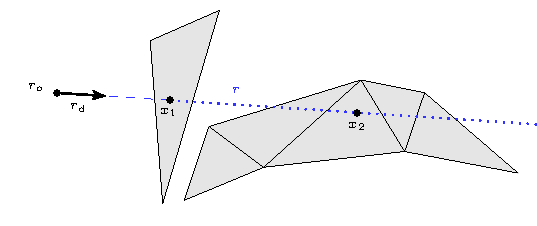
\includegraphics{ray_tracing_1.pdf}
    \end{figure}
    \begin{itemize}
      \item determine the visibility of surfaces in a scene from an origin
      \item use a ray to compute nearest intersections
    \end{itemize}
  \end{frame}
  \begin{frame}
    \frametitle{Ray Tracing Background}
    \begin{figure}[H]
      \center
      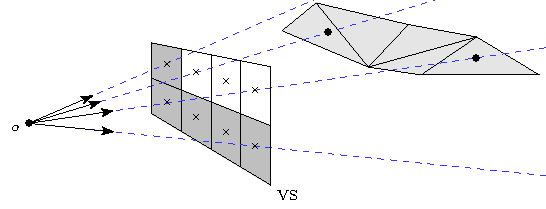
\includegraphics{ray_tracing_2.pdf}
    \end{figure}
    \begin{itemize}
      \item trace a bunch of rays for every pixel
      \item apply shading and show the result
    \end{itemize}
  \end{frame}
  % section ray_tracing_background (end)

  \section{Starting Point} % (fold)
  \label{sec:starting_point}
  \begin{frame}
    \frametitle{Starting Point}
    Group of 3 People:
    \begin{itemize}
    \setlength\itemsep{1.5em}
      \item different background and knowledge base
      \item different hardware
      \begin{itemize}
        \item for example: ordinary laptops, non-ordinary laptops, desktop computer
      \end{itemize}
      \item different operating systems
      \begin{itemize}
        \item for example: Windows 7, macOS, Ubuntu, Arch Linux
      \end{itemize}
    \end{itemize}
  \end{frame}
  % section starting_point (end)

  \section{Setting up the Environment} % (fold)
  \label{sec:setting_up_the_environment}
  \begin{frame}
    \frametitle{Setting up the Environment}
    \begin{itemize}
    \setlength\itemsep{1.5em}
      \item tools known from the lecture:
      \begin{itemize}
        \item Intel C++ compiler, git, CMake, clang-format, etc...
      \end{itemize}
      \item choice of code editor:
      \begin{itemize}
        \item Sublime Text 3 with given configurations for C++ and clang-format
      \end{itemize}
      \item C++ coding style
      \begin{itemize}
        \item Google C++ style guide with some minor changes
      \end{itemize}
    \end{itemize}
  \end{frame}
  \begin{frame}
    \frametitle{Setting up the Environment}
    \begin{itemize}
    \setlength\itemsep{1.1em}
      \item git branching model
      \item git commit message style
      \item learning modern CMake
      \item installing GLUT-library in Windows 7
    \end{itemize}
  \end{frame}
  \begin{frame}
    \frametitle{Setting up the Environment}
    \begin{itemize}
    \setlength\itemsep{1.1em}
      \item communication via E-Mail and GitLab-Issue system
      \item additional meeting every week
      \item one feature per group member per week
    \end{itemize}
  \end{frame}
  % section setting_up_the_environment (end)

  \section{Implementation} % (fold)
  \label{sec:implementation}
  \begin{frame}
    \frametitle{Implementation}
    \begin{itemize}
    \setlength\itemsep{1.1em}
      \item OpenGL scene viewer with user interaction
      \item scene loader: STL-files, OBJ-files
      \item camera
      \item FPS measurement
      % \item naive ray tracing
      % \item BVH rendering
      % \item anti-aliasing
    \end{itemize}
  \end{frame}
  \begin{frame}
    \frametitle{Naive Ray Tracing}
    \begin{figure}[H]
      \center
      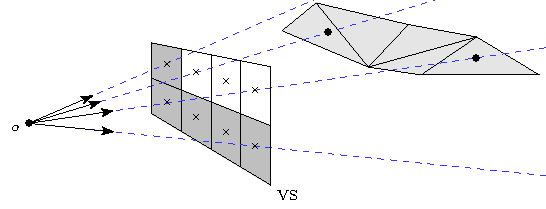
\includegraphics{ray_tracing_2.pdf}
    \end{figure}
    \begin{itemize}
      \item for each ray check existance of intersection with each primitive
    \end{itemize}
  \end{frame}
  \begin{frame}
    \frametitle{Morton Code}
    \begin{figure}[H]
      \center
      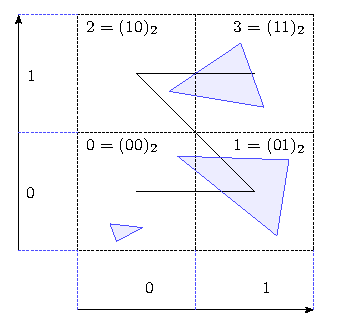
\includegraphics{morton_code_1_.pdf}
    \end{figure}
    \begin{itemize}
      \item enclose scene in a bounding box
      \item order primitives of scene with respect to their morton code
    \end{itemize}
  \end{frame}
  \begin{frame}
    \frametitle{Bounding Volume Hierarchy (BVH)}
    \begin{figure}[H]
      \center
      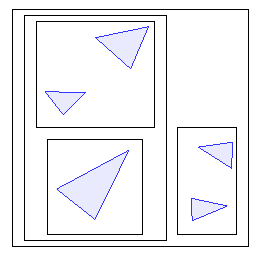
\includegraphics{bvh_1.pdf}
    \end{figure}
    \begin{itemize}
      \item use morton code to build a tree structure
      \item enclose primitives of every node in a bounding box
    \end{itemize}
  \end{frame}
  \begin{frame}
    \frametitle{Parallelization}
    naive ray tracing:
    \begin{itemize}
      \item static parallelization over pixels
    \end{itemize}
    \bigskip
    BVH ray tracing:
    \begin{itemize}
      \item FPS depends on camera position and screen pixel
      \item use blocking principle with block size of 8
      \item dynamic scheduling in for loop
    \end{itemize}
  \end{frame}
  \begin{frame}
    \frametitle{Vectorization}
    Now:
    \begin{itemize}
      \item done by compiler through Eigen-library
    \end{itemize}
    \bigskip
    Future:
    \begin{itemize}
      \item vectorization of intersection computation
      \item vectorization of BVH traversal
      \item vectorized random number generation
    \end{itemize}
  \end{frame}
  % section implementation (end)

  \section{Serialization / Deserialization} % (fold)
  \label{sec:camera_paths}
  \begin{frame}
    \frametitle{Serialization / Deserialization}
    Goal:
    \begin{itemize}
      \item Track user camera movement over time while running spray
      \item Serialize the movement by storing camera parameters and time data externally
      \item Deserialize by reading the parameters back into the camera object
      \item Render the recorded camera movement over time
    \end{itemize}
    \vskip1ex
    \begin{center}
        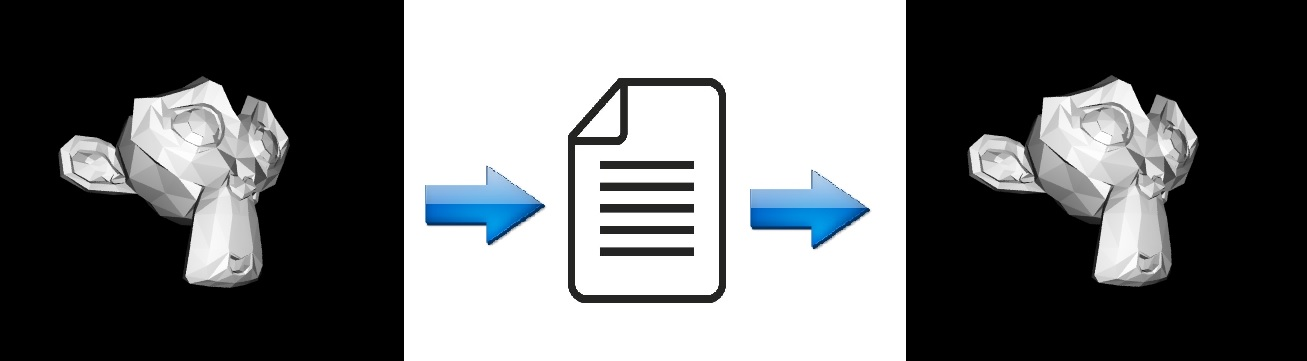
\includegraphics[width=70mm]{monkeyprocess.jpg}
    \end{center}
  \end{frame}

  \begin{frame}
    \frametitle{Serialization / Deserialization}
    Limitation:
    \begin{itemize}
      \item Frame resolution is bounded by the rendering speed during recording; playback is always as choppy as the rendering was on the machine that recorded it.
    \end{itemize}
    \bigskip
    Solution:
    \begin{itemize}
      \item Interpolate between recorded camera parameters, display extra frames for a smoothing effect.
    \end{itemize}
  \end{frame}
  % section camera_paths (end)

  \section{More Future Work} % (fold)
  \label{sec:more_future_work}
  \begin{frame}
    \frametitle{More Future Work}
    \begin{itemize}
    \setlength\itemsep{1.1em}
      \item template-based library
      \item more objective measurements
      \item implementing physicaly based shading of primitives
      \item adding smoothed particle hydrodynamics
      \item and even more...
    \end{itemize}
  \end{frame}
  % section more_future_work (end)

  \begin{frame}
    \vfill
    \center
    Thank you very much for your attention!
    \vfill
  \end{frame}
\end{document}
